\section{Single speaker source}
This section aims to introduce and analyse the fundamental for a single source, by analyse the behaviour of a line source shaped as the diaphragm. The pressure around the speaker will be analysed analytically, to determine the radiation of a single speaker from \SI{60}{\hertz} and upwards. The \SI{60}{\hertz} lower limit enable the simulation to be validated by measurement in the AAU anacoid chamber and is a used lower limit for the low/mid driver in some line source array.  The analyse shall end out with a limited frequency range, where the directivity have to be controlled.

\subsection{Pressure analysis around a single source}
To characterised the directions properties of a speaker unit, the source will be modulated as three line source shaped as the diaphragm of a speaker. To modulated the diaphragm, a continues line source will be analysed and explained in this section. The analysis of a continues line source built on a thin cylindrical source of length $L$, and have radius $a$. The line source is considered as many small sources which vibrate radially, where the vibration speed is complex and modelled as  

\begin{equation}
u = \text{\textit{{\LARGE u}}}_{0} \cdot exp(j \omega t)
\end{equation}

    \startexplain
        \explain{$\text{\textit{{\LARGE u}}}_{0}$ is the Amplitude}{\si{\ohm}}
        \explain{$R_F$ is a resistor in the feedback circuit}{\si{\ohm}}
    \stopexplain







\autoref{fig:single_speaker_model} shows the model of the speaker unit.


\begin{figure}[htbp]
	\centering
	\begin{picture}(0,0)%
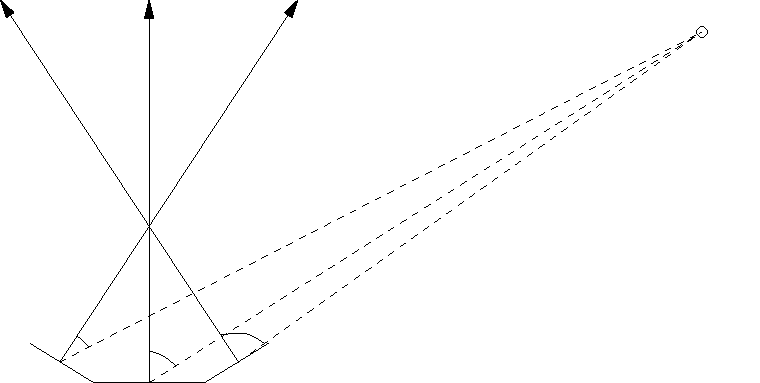
\includegraphics{speaker_model.pdf}%
\end{picture}%
\setlength{\unitlength}{746sp}%
%
\begingroup\makeatletter\ifx\SetFigFont\undefined%
\gdef\SetFigFont#1#2#3#4#5{%
  \reset@font\fontsize{#1}{#2pt}%
  \fontfamily{#3}\fontseries{#4}\fontshape{#5}%
  \selectfont}%
\fi\endgroup%
\begin{picture}(32123,16224)(-6311,827)
\put(24121,15599){P(r,$\theta$,t)}%
\put(-2744,2684){$\theta$}%
\put(496,2234){$\theta$}%
\put(4411,3089){$\theta$}%
\end{picture}%
	\caption{The model of a speaker unit}
		\label{fig:single_speaker_model}
\end{figure}





\begin{equation}
p(r,\theta ,t)=\frac{j}{2}*\rho_{0}c  \text{\textit{{\LARGE u}}}_{0}\frac{a}{r}kL\left ( \frac{sin(\frac{1}{2}kLsin(\theta ))}{\frac{1}{2}kLsin(\theta )} \right )e^{j(\omega t-kr)}
\end{equation}
